\chapter{Máquina de Turing}

Fue diseñada por el matematic ingles Alan M. Turing en 1936. consta de una cinta infinita, en los que podemos ubicar a la cadena a procesasr en cualquier celda la cual le da una capacidad ilimitada de almacenamiento.

Tinene un cabezal que es de lectura y escritura. Usa dos alfabetos, el alfabeto de entrada y el de la cinta.\\
En la función de transición se considera el desplazamiento.

Los autómatas finitos son menos potentes que los autómatas a pila con respecto a la capacidad de aceptar lenguajes. Las máquinas de Turing son más generales al poder aceptar lenguajes regulares como lenguajes libres de contexto u otros lenguajes.

\section{Arquitectura de una MT}
%grafico1
\begin{figure}[h!]
\centering
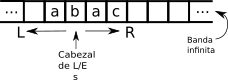
\includegraphics[width=0.3\textwidth]{img_19_1.png}
\caption{Máquina de Turing}\label{img_19_1}
\end{figure}

\textbf{Definición: }Una máquina de Turing es una séptupla
$$M=(S,\Sigma,\Gamma,s,\not b, F,\delta)$$
\begin{tabular}{rl}
$S$			&	: Conjunto finito de estados	\\
$\Sigma$	&	: Alfabeto de entrada	\\
$\Gamma$	&	: Alfabeto de la cinto	\\
s			&	: Estado inicial $s\in S$	\\
$\not b$	&	: El símbolo blanco $(\not b \not\in\Sigma )$	\\
F			&	: Conjunto de estados de aceptación $(F\subseteq S)$	\\
$\delta$	&	: $S\times\Sigma\rightarrow S\times\Gamma\times \downlegend{D}{desplaza}$; $D=\{L,R\}$
\end{tabular}

\begin{enumerate}
\item El valor inicial de todas las celda es $\not b$.
\item Permitimos que $\Sigma \in \Gamma -\{\not b\}$.
\item $\delta$ transforma pares en ternas
$$(\downlegend{p}{(a)},\downlegend{\sigma}{(b)})\rightarrow (\downlegend{q}{(c)},\downlegend{t}{(d)},\downlegend{X}{(e)})$$
(a)estado actual, (b)símbolo actual, (c)estado siguiente, (d)símbolo de la cinta, (e)desplazamiento
\end{enumerate}

\textbf{Ejemplo: }La transición $\delta(q_i,a)=(q_s,b,R)$, provoca que la máquina de Turing pase de la configuración(Fig \ref{img_19_2}):
%grafico 2
\begin{figure}[h!]
\centering
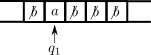
\includegraphics[width=0.2\textwidth]{img_19_2.png}
\caption{Configuración inicial}\label{img_19_2}
\end{figure}

A la siguiente configuración(Fig \ref{img_19_3}):
%grafico 3
\begin{figure}[h!]
\centering
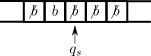
\includegraphics[width=0.2\textwidth]{img_19_3.png}
\caption{Configuración final}\label{img_19_3}
\end{figure}

\textbf{OBS: }$\delta$ no necesariamente está definido para algún par de $S\times\Sigma$.
\section{Etapas en el Proceso de una Cadena}
\textbf{Ejemplo: }Sea la MT definida mediante:
\begin{align*}
S	&=\{q_1,q_2\}	\\
\Sigma	&=\{a,b\}	\\
\Gamma	&=\{a,b,\not b\}	\\
F		&=\{q_2\}	\\
s		&= q_1
\intertext{$\delta$ está dada por}
\delta(q_1,a)	&=(q_1,a,R)	\\
\delta(q_1,b)	&=(q_1,a,R)	\\
\delta(q_1,\not b)	&=(q_2,\not b,L)
\intertext{Supongamos que se tiene $w=abba$. La configuracion seria(Fig \ref{img_19_4}): }
\end{align*}
%grafico 4
\begin{figure}[h!]
\centering
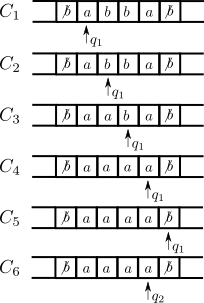
\includegraphics[width=0.25\textwidth]{img_19_4.png}
\caption{Llega a un estado de aceptación, por tanto se acepta $w$}\label{img_19_4}
\end{figure}


\section{Representación para la configuración de una MT}
Podemos utilizar dos notaciones:

\textbf{Notación 1: }$(q_1,w_1\sigma w_2)$

\begin{tabular}{rl}
$q_1$	&: Estado actual	\\
$w_1$	&: Cadena que precede al símbolo apuntado por la cabeza de L/E	\\
$\sigma$	&: Símbolo al que apunta el cabezal.	\\
$w_2$	&: Subcadena que está por procesar.
\end{tabular}

\textbf{Configuración: }Se tiene lo siguiente:
\begin{align*}
C_1	&\quad(q_1,\not b\underline{a}bba)	\\
C_2	&\quad(q_1, a\underline{b}ba)	\\
C_3	&\quad(q_1, aa\underline{b}a)	\\
C_4	&\quad(q_1,aaa\underline{a}\not b)	\\
C_5	&\quad(q_1,aaaa\underline{\not b}\not b)	\\
C_6	&\quad(q_2, aaa\underline{a}\not b)
\end{align*}
\textbf{Notación 2: }$a_1...a_{k-1}q_1a_ka_{k+1}...a_n$ es la representación de $(q_1,a_1...a_{k-1}a_k...a_n)$ donde $q_1$ es el estado actual.
\begin{align*}
\intertext{Configuración: }
C_1	&\quad \not bq_1abba	\\
C_2	&\quad aq_1bba	\\
C_3	&\quad aaq_1ba	\\
C_4	&\quad aaaq_1a\not b	\\
C_5	&\quad aaaaq_1\not b\not b	\\
C_6	&\quad aaaq_2a\not b
\end{align*}
\textbf{OBS: }Se utiliza el símbolo $\vdash$ para representar el paso de una configuración a otra.
$$(q_1,\not b\underline{a}bba)\vdash(q_1,a\underline{b}ba)\vdash...\vdash(q_2,aaa\underline{a}\not b)$$
Recordar que:
\begin{align*}
\vdash^* \qquad \mbox{significa ''0 a mas''}	\\
\vdash^+ \qquad \mbox{significa ''1 a mas''}
\end{align*}
\textbf{Ejemplo: }Dada la MT.
\begin{align*}
S		&=\{ q_1,q_2,q_3\}	\\
\Sigma	&=\{a,b\}	\\
\Gamma	&=\{a,b,\not b\}	\\
F		&=\{q_3\}	\\
s		&= q_3
\intertext{$\delta$ viene definida por: }
\delta(q_1,a)		&=	(q_1, a) L	\\
\delta(q_1,b)		&=	(q_1,b) L	\\
\delta(q_1,\not b)	&=	(q_2,\not b)R	\\
\delta(q_2,a)		&=	(q_3,a)L	\\
\delta(q_2,b)		&=	(q_3,b)L	\\
\delta(q_2,\not b)	&=	(q_3,\not b)L	\\
\intertext{Procesar $w=aababb$ mediante transiciones}
\end{align*}
$$(q_1,\underline{a}ababb)\vdash (q_1,\underline{\not b}aababb)\vdash(q_2, \not b\underline{a}ababb)\vdash (q_3, \underline{\not b}aababb)$$
Cuando $\delta(q,a)$ está indefinida y la configuración de la MT es $(q,w_1qw_2)$ es imposible que pase a otra. Entonces se dice que la MT está parada.

La MT se parará siempre que llegue a un estado d aceptación.

\textbf{Definición: }La secuencia de todos los movimientos que conducen a una configuración parada se llama \textbf{computación}.

\textbf{OBS: }También es posible que la MT se mueva indefinidamente con la cabeza de L/E desplazándose de izquierda a derecha alternativamente.

\textbf{Notación: }
\begin{align*}
(q_1,w_1\sigma w_2)&\vdash^* \infty	\\
w_1q_1\sigma w_2	&\vdash^* \infty
\intertext{Significa que la MT nunca se detendrá.}
\end{align*}

\section{Paso Computacional}
El paso de una CI a otra a través de una transición por $\delta$ se llama paso computacional y se denota por:
$$u_1qu_2\vdash v_1q_2v_2$$

\section{Cómputos Especiales}
Al procesar una cadena  de entrada hay dos casos especiales.
\begin{enumerate}
\item El cómputo no termina porque entró a un bucle infinito. $u_1s_1u_2 \vdash^* \infty$.
\item El cómputo termina porque en determinado momento no hay una transición definida.
\end{enumerate}

\section{Lenguaje Aceptado por una MT}
Una cadena $w\in\Sigma^*$ es aceptado por una MT si el cómputo que parte de una configuración inicia $s_0w$ termina en una CI $\alpha_1s\alpha_2$, $s\in F$ en la cual la MT se detiene por completo.
$$L(M)=\{w\in\Sigma^*/s_0w\vdash^* \alpha_1s\alpha_2, s\in F, \alpha_1\alpha_2 \in \Gamma^*\}$$

\textbf{Ejemplo: }Dibuje la tabla de transición para una MT que obtenga el complemento binario de un número binario almacenado en la cinta.

Sea la MT definida por:
\begin{align*}
\Sigma	&=\{0,1\}	\\
\Gamma	&=\{0,1,\not b\}	\\
S		&=\{s_0,s_1\}	\\
s		&=s_0	\\
F		&=\{s_1\}
\end{align*}
\begin{center}
\begin{tabular}{c|c|c|c}
		&0			&1			&$\not b$	\\ \hline
$s_0$	&$s_01D$	&$s_00D$		&$s_1\not bI$
\end{tabular}
\end{center}